\chapter{Ejercicio 2}

\section{Actividad 1}

\textbf{A)} Expresar la Ecuación Diferencial (ED) que describe el circuito, y con ello, definir un
Sistema en tiempo continuo con entrada x(t) = v(t) y salida y(t) = i(t) , con condiciones
Iniciales genérica (CI).

\begin{figure}[H]
  \centering
  \begin{circuitikz}[american voltages]
    \node at (-3,1) {ENTRADA};
    \node at (-3,0) {$x(t) = v(t)$};
    
    \draw (-1,-1) rectangle (3.5,2.5);

    \draw (-0.5,1.5) to[R=$R$] (2,1.5)
          to[C=$C$] (2,-0.5) -- (-0.5,-0.5);
    
    \draw[->] (-4, 0.5) -- (-1,0.5);

    \node at (6,1) {SALIDA};
    \node at (6,0) {$y(t) = i(t)$};
    
    \draw[->] (3.5,0.5) -- (6,0.5);
  \end{circuitikz}
\end{figure}

Para plantear la EDO es necesario plantear ley de kirchoff

$$v(t) = R \cdot i(t) + \dfrac{1}{C} \cdot \int i(t) dt$$

Ahora derivamos para conseguir la expresion buscada

$$\dfrac{d v(t)}{dt} = R \dfrac{d i(t)}{dt} + \dfrac{1}{C} \cdot i(t)$$

Dividimos todo por $R$ para normalizar la ecuacion

$$\dfrac{d i(t)}{dt} + \dfrac{1}{RC} \cdot i(t) = \dfrac{1}{R} \cdot \dfrac{d v(t)}{dt}$$

$$y'(t) + \dfrac{1}{RC} \cdot y(t) = \dfrac{1}{R} \cdot x'(t)$$

Para el circuito de segundo orden:

\begin{figure}[H]
  \centering
  \begin{circuitikz}[american voltages]
    \node at (-3,1) {ENTRADA};
    \node at (-3,0) {$x(t) = v(t)$};
    
    \draw (-1,-1) rectangle (3.5,2.5);

    \draw (-0.5,1.5) to[R=$R$] (1.25,1.5) to[L=$L$] (2.3,1.5)
          to[C=$C$] (2.3,-0.5) -- (-0.5,-0.5);
    
    \draw[->] (-4, 0.5) -- (-1,0.5);

    \node at (6,1) {SALIDA};
    \node at (6,0) {$y(t) = i(t)$};
    
    \draw[->] (4,0.5) -- (6,0.5);
  \end{circuitikz}
\end{figure}

Siguiendo con el mismo procedimiento

$$v(t) = R \cdot i(t) + L \cdot \dfrac{d i(t)}{dt} + \dfrac{1}{C} \cdot \int i(t) dt$$

$$\dfrac{d v(t)}{dt} = R \cdot \dfrac{d i(t)}{dt} + L \cdot \dfrac{d^2 i(t)}{dt^2} + \dfrac{1}{C} \cdot i(t)$$

$$\dfrac{d^2 i(t)}{dt^2} +  \dfrac{R}{L} \cdot \dfrac{d i(t)}{dt} + \dfrac{1}{LC} \cdot i(t) = \dfrac{1}{L} \cdot \dfrac{d v(t)}{dt} $$

$$y''(t) + \dfrac{R}{L} \cdot y'(t) + \dfrac{1}{LC} \cdot y(t) = \dfrac{1}{L} \cdot x'$$

\textbf{B)}Usar la transformada de Laplace para sintetizar el sistema en la expresión

Primero sintetizamos la ecuacion correspondiente al circuito de primer orden

$$\mathscr{L}[y'(t)] = sY(s) - y(0)$$

$$\mathscr{L}[y(t)] = Y(s)$$

$$\mathscr{L}[x'(t)] = sX(s) - x(0)$$

Quedando la ecuacion

$$sY(s) - y(0) + \dfrac{1}{RC} \cdot Y(s) = \dfrac{1}{R} \cdot (sX(s) - x(0))$$

$$Y(s) (s + \dfrac{1}{rc}) = \dfrac{1}{R} \cdot sX(s) - \dfrac{1}{R} x(0) + y(0)$$

$$Y(s) = X(s)  \dfrac{\dfrac{s}{R}}{s + \dfrac {1}{RC}} + \dfrac{1}{(s + \dfrac{1}{RC})} [y(0) - x(0) \dfrac{1}{R}]$$

Ya nos queda sintetizado a la expresion

$$Y(s) = X(s) \cdot H(s) + F(s,CI)$$

Ahora para el circuito de segundo orden, primero debemos definir la transformada para la segunda derivada

$$\mathscr{L}[y''(t)] = s^2Y(s) - sy(0) - y'(0)$$

Quedando la ecuacion sintetizada

$$ s^2Y(s) - s y(0) - y'(0) + \dfrac{R}{L} (sY(s) - y(0)) + \dfrac{1}{LC} \cdot Y(s) = \dfrac{1}{L} \cdot (sX(s) - x(0))$$

$$ Y(s) (s^2 + \dfrac{R}{L} s + \dfrac{1}{LC}) = X(s) \dfrac{s}{L} - x(0) \dfrac{1}{L} + s y(0) + y'(0) + \dfrac{R}{L} y(0)$$

$$ Y(s) = X(s) \dfrac{\dfrac{s}{L}}{s^2 + \dfrac{R}{L} s + \dfrac{1}{LC}} + \dfrac{1}{s^2 + \dfrac{R}{L} s + \dfrac{1}{LC}} [s y(0) + y'(0) + \dfrac{R}{L} y(0) - x(0) \dfrac{1}{L}]$$

\textbf{C)} Escribir un diagrama de Bloques en la variable compleja S que determine al Sistema.

El diagrama de bloques que describe a la ecuacion de primer orden es:

\begin{figure}[H]
  \centering
  \begin{circuitikz}
    \node at (-2.5,1) {$X(s)$};
    \draw[->] (-3,0.5) -- (0,0.5);

    \draw (0,1) rectangle (1,0);

    \node at (0.5,0.5) {$H(s)$};
  
    \draw (1,0.5) -- (3,0.5);
    \draw[->] (3,0.5) -- (3,-0.5);

    \node at (-2.5,-2) {$F(s,CI)$};
    \draw[->] (-3,-2.5) -- (0,-2.5);

    \draw (0,-1.87) rectangle (1.25,-3.12);
    
    \draw (1.25,-2.5) -- (3,-2.5);
    \draw[->] (3,-2.5) -- (3,-1);

    \node[scale=0.7] at (0.625,-2.475) {$\dfrac{1}{s+\dfrac{1}{RC}}$};

    \draw (3,-0.75) circle (0.25cm);

    \node at (3,-0.75) {+};

    \draw[->] (3.25,-0.75) -- (4.25,-0.75);
    \node at (4,-0.25) {$Y(s)$};
  \end{circuitikz}
\end{figure}

Por otro lado el que describe a la ecuacion de segundo orden

\begin{figure}[H]
  \centering
  \begin{circuitikz}
    \node at (-2.5,1) {$X(s)$};
    \draw[->] (-3,0.5) -- (0,0.5);

    \draw (0,1) rectangle (1,0);

    \node at (0.5,0.5) {$H(s)$};
  
    \draw (1,0.5) -- (3,0.5);
    \draw[->] (3,0.5) -- (3,-0.5);

    \node at (-2.5,-2) {$F(s,CI)$};
    \draw[->] (-3,-2.5) -- (0,-2.5);

    \draw (0,-1.87) rectangle (1.25,-3.12);
    
    \draw (1.25,-2.5) -- (3,-2.5);
    \draw[->] (3,-2.5) -- (3,-1);

    \node[scale=0.45] at (0.625,-2.475) {$\dfrac{\dfrac{s}{L}}{s^2+\dfrac{R}{L}s+\dfrac{1}{LC}}$};

    \draw (3,-0.75) circle (0.25cm);

    \node at (3,-0.75) {+};

    \draw[->] (3.25,-0.75) -- (4.25,-0.75);
    \node at (4,-0.25) {$Y(s)$};
  \end{circuitikz}
\end{figure}

\textbf{D)} Graficar en el plano $S$ polos y ceros de $H(s)$.

Para el caso de primer orden

$$H(s) = \dfrac{\dfrac{s}{R}}{s + \dfrac{1}{RC}}$$

Donde el unico polo se encuentra en $s=-\dfrac{1}{RC}$ y el cero en $s=0$.

$R = 3$, $C = \dfrac{1}{2}$, $L = 1$.

El polo con estos datos seria $s=-\dfrac{2}{3}$

\begin{figure}[H]
  \centering
  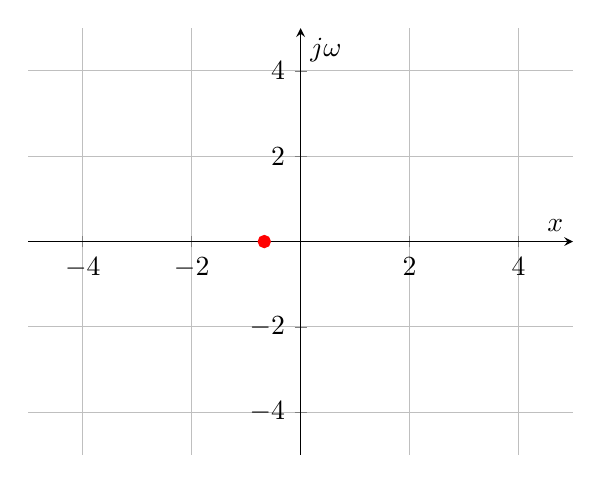
\begin{tikzpicture}
    \begin{axis}[
        axis lines=middle,
        xlabel={$x$},
        ylabel={$j\omega$},  
        grid=both,
        width=8.5cm,
        height=7cm,
        ymin=-5, ymax=5,
        xmin=-5, xmax=5,
      ]
      \addplot[red, thick, mark=*] coordinates {(-2/3,0)};
    \end{axis}
  \end{tikzpicture}
\end{figure}

Para la ecuacion de segundo orden 

$$H(s) = \dfrac{\dfrac{s}{L}}{s^2 + \dfrac{R}{L} s + \dfrac{1}{LC}}$$

Y los polos se encontrarian en $s_n=\dfrac{-\dfrac{R}{L} \pm \sqrt{\dfrac{R}{L}^2-\dfrac{4}{LC}}}{2}$

Donde reemplazando con los valores previamente dados, los polos quedarian en $(-1,0)$ y $(-2,0)$.

\begin{figure}[H]
  \centering
  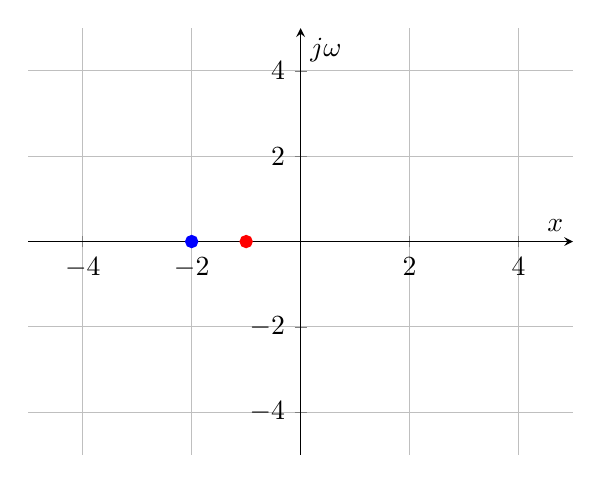
\begin{tikzpicture}
    \begin{axis}[
        axis lines=middle,
        xlabel={$x$},
        ylabel={$j\omega$},  
        grid=both,
        width=8.5cm,
        height=7cm,
        ymin=-5, ymax=5,
        xmin=-5, xmax=5,
      ]
      \addplot[red, thick, mark=*] coordinates {(-1,0)};
      \addplot[blue, thick, mark=*] coordinates{(-2,0)};
    \end{axis}
  \end{tikzpicture}
\end{figure}

